\documentclass[11pt]{article}

\usepackage[letterpaper,left=1.6in,right=1.6in,top=1.2in,bottom=1.2in]{geometry}

\usepackage[T1]{fontenc}
\usepackage[utf8]{inputenc}

\usepackage{lmodern}
\usepackage{amssymb,amsmath}
\usepackage{algorithm,algorithmic}
\usepackage{hyperref}
\usepackage{graphicx}
\usepackage{listings}
\usepackage[11pt]{moresize}

\setcounter{secnumdepth}{0}

%\usepackage[vlined]{algorithm2e}
\usepackage{algorithm,algorithmic}
\usepackage{paralist}
\usepackage{tikz}
\usepackage{xcolor,colortbl}

\begin{document}
\lstset{language=Java}
\begin{center}
\begin{HUGE}{\bf A6 - Shipping Game}\\ \end{HUGE}
\vspace{3mm}
\begin{LARGE} By Michael Patashnik and the CS2110 Course Staff\\ \end{LARGE}
\vspace{7mm}
\begin{LARGE} Contents\\ \end{LARGE}
\noindent\rule{8cm}{0.4pt}
\begin{enumerate} \begin{large}
\item Heap
\item Game Overview
\item Installation
\item Using the GUI
\item Class Explanation
\item Your Tasks
\item Concurrency
\item Project Schedule
\end{large}\end{enumerate}
\end{center}
\newpage

\section{1. Heaps}
As a prologue to Shipping Game, you have to implement a Heap. Heaps are
extremely useful data structures that play a vital role in many graph
algorithms, including Dijkstra's Algorithm.

Write a class that implements the MinHeap interface and sticks to the given time
bounds. To test your code, run the HeapTester main method with your heap
implementation classname as an argument. If all of the tests pass, then you're
ready to go!

Due to the nature of the project, writing the Heap is a very small part of the
project from a conceptual sense. Try to have the heap finished \textbf{early}
(see section 8) after starting the project, so that you have enough time to work
on the rest of the project.

TODO: Expand on this section.



\newpage
\section{2. Game Overview}
In Shipping Game (less descriptive name pending) you play the part of a shipping
company engineer who makes sure that deliveries get where they're going in a
timely fashion. In an instance of Shipping Game, you are presented with an
undirected, weighted graph that represents the world. The nodes in this graph
are cities where parcels are picked up from or dropped off to, and the edges are
highways that connect the cities. Parcels are distributed around the map, each
with a starting location (a city in the map) and a delivery destination (a
different city in the map).\\
\centerline{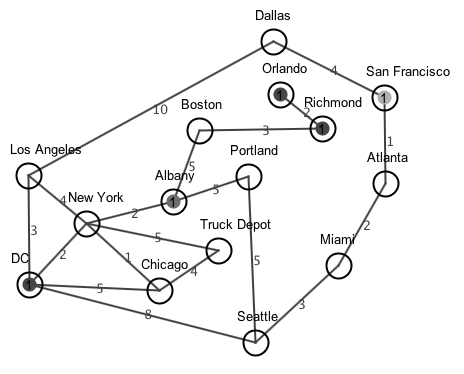
\includegraphics[scale=0.8]{map1.png}}\\
Cities in the map are labeled with their name, highways with their length. The
smaller filled-in circles that appear in some cities are parcels that need to be
picked up and delivered elsewhere on the map.\\

In order to accomplish this task, you have a fleet of trucks that you are able
to control. At the beginning of the game you have the option to give your trucks
instructions. Additionally, whenever a truck reaches an important point, such as
reaching its destination after traveling a highway, it will let you know so you
can give it additional instruction. All Trucks begin the game on the Truck Depot
city (there will be exactly one truck depot in every map) and must return there
after delivering all parcels for the game to end.

\newpage
\section{3. Installation and Running}
\subsection{Installation}
The code for this project is provided as a .jar file, without source-attachment.
Various data files are provided as text files in folders.
\begin{enumerate}
\item Create a new Java project in Eclipse, name it A6.
\item Download ShippingGame.jar and all of the data folders, drag them into your
	A6 folder. Don't change the names of any of the folders or the code won't be
	able to find the data.
\item Right click A6 --> Build Path --> Add External Archives --> Select
	ShippingGame.jar and click Open.
\item Right click A6 -> Build Path --> Configure Build Path... --> Expand
	ShippingGame.jar by clicking on the triangle to the left of it --> Select
	Javadoc Location --> Click Edit... --> Select "Javadoc URL" --> Click
	Browse... --> Select the "doc" folder (don't expand it) and click Open,
	Click Ok, Click Ok.
\item Create a package in the src folder (right click src --> new... -> package)
	called \textbf{student}. All code you write for this project must be in the
	student package.
\item Create a Class in the student package (called whatever you like) that
	extends \textbf{game.Manager}. Notably, you can't call it Manager. This is
	your manager class, and is your main submission.
\end{enumerate}

\subsection{Running}
\begin{enumerate}
\item Select A6 -> Run As... --> Run Configurations... --> New Launch
	Configuration (blank page with star in top left)
\item Click Search... next to Main class --> Select game.main
\item Switch to the Arguments tab --> Enter the name of your manager class that
	you created in the student class in the top text box. No .java necessary,
	just the name of the class.
\item Click run.
\item From here on out, the settings are saved, so you can simply run the
	project by clicking the green run button as usual.
\end{enumerate}

\subsection{Arguments}
You can provide additional arguments to the runner to have it do different
things. All argument combinations have to start with the name of your manager.
With just the manager classname provided, the game will launch in GUI mode.
There are no other applicable arguments for this mode. Any other combination of
arguments will launch the game in GameRunner mode instead, where the game will
automatically run your manager on a sequence of maps. 

To run GameRunner on a series of seeds <seed1> <seed2> <seed3> such as $15,
12345, 907230587$, use each seed as an argument, separated by a space. (replace
MyManager with the name of your Manager):
\begin{center}
MyManager 15 12345 907230587
\end{center}
To run GameRunner on a series of $n$ random seeds, use the $-r$ flag, followed
by the number of random seeds to run (replace MyManager with the name of your
Manager). For example, to run your manager on 10 random seeds:
\begin{center}
MyManager -r 10
\end{center}
The GameRunner mode includes the GUI to show the progression of the run games.
It also prints output of the games to the console. If you would like to just see
the output and not show the GUI (headless), add the $-h$ tag. Thus, either:
\begin{center}
MyManager -h 15 12345 907230587
\end{center}
or
\begin{center}
MyManager -h -r 10
\end{center}
\begin{figure}[h]
\centerline{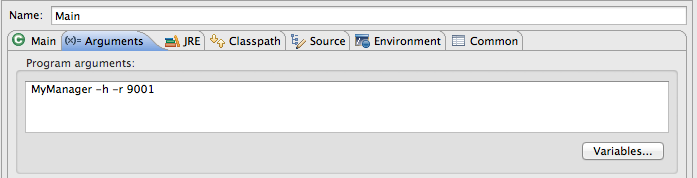
\includegraphics[scale=0.65]{args.png}} 
\caption{\em{Running MyManager in headless mode on 9001 random seeds.}}
\end{figure}


\newpage
\section{4. Using the GUI}
\begin{figure}[h]
\centerline{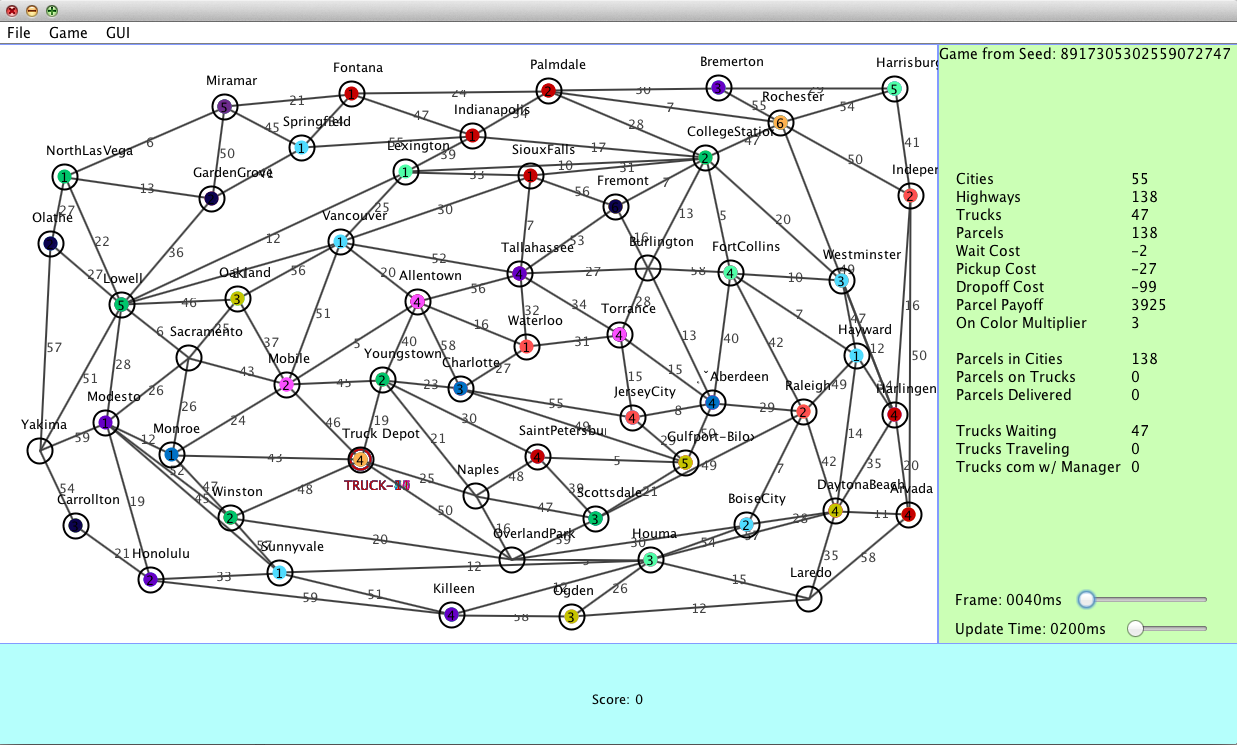
\includegraphics[scale=0.45]{gui.png}} 
\caption{\em{The Shipping Game GUI. Now with 50\% less (visual) sugar!}}
\end{figure}

Assuming the installation process went correctly and you've created a class that
extends manager, you should be able to run the main class and see the above gui.
{\em(Note, generated map may be different than pictured above)}. In addition to
being fully resizable, the gui has a number of features for your use. All of the
cities (nodes) on the board are draggable to allow you to make the graph look
cleaner, but note that this is a purely visual change and has no impact on the
underlying board state.

\subsection{4a. Menu Bar}
\begin{itemize}
\item File...
\begin{itemize}
\item Open... - Opens a JFileChooser rooted at the data/maps directory. Allows
	you to choose a map (in JSON format) to load on the gui.
\item Quit - Closes the current gui and quits the program.
\end{itemize}
\item Game...
\begin{itemize}
\item Start - begins the currently displayed game. Clicking this additional
	times after the game has begun does nothing.
\item Reset - Resets the currently displayed game to its pre-start state. Only
	available once the game has begun.
\item New Random Map... - Generates a new random map with the seed given to the
	popup window. If a non-digit character is provided, asks for a new seed.
	Exit this option by clicking cancel on the popup window.
\item Print Game JSON - prints a JSON string representing this game to the
	eclipse console. Useful to save an interesting board by resetting it,
	printing the game JSON and creating a new text file in the data/maps
	directory with the game JSON as its contents.
\end{itemize}
\item GUI...
\begin{itemize}
\item Repaint - repaints the gui. Try clicking this if the gui looks strange
	before trying other solutions.
\item Edge Coloring - controls how edges are colored on the gui.
\begin{itemize}
\item Default - colors all edges as a dark gray
\item Highlight-Travel - colors edges that are currently being traveled by a
	truck as red, others as dark gray. Will draw all edges as dark gray if the
	game hasn't started yet or is over (as no trucks are currently traveling).
\item Distance Gradient - colors edges by a linear interpolation from light to
	dark, based on their weights. Shorter (lighter) edges are painted in a
	lighter color, and longer (heavier) edges are painted in a  darker color.
\end{itemize}
\end{itemize}
\end{itemize}

\subsection{4b. Info Panel}
The panel on the right is the info panel - it displays useful information about
the currently displayed game.  The top block of data is static data - it will
not change as the game runs.
\begin{itemize}
\item Game From... - A description of the current game - either from seed, from
	file, or custom
\item Cities - the number of nodes
\item Highways - the number of edges
\item Trucks - the number of available trucks
\item Parcels - the total number of parcels, including delivered parcels
\item Wait Cost - the cost (per frame) of a truck doing nothing
\item Pickup Cost - the singleton cost of a truck picking up a parcel
\item Dropoff Cost - the singleton cost of a truck dropping off a parcel
\item Parcel Payoff - the singleton value of dropping off a parcel at its
	location
\item On Color Multiplier - the multiplier applied to the parcel payoff if the
	delivering truck and the parcel share a color.
\end{itemize}

The next two blocks are non-static data. They are changed through the course of
the game.
\begin{itemize}
\item Parcels in Cities - the number of undelivered parcels that are not
	currently held by trucks (thus on cities)
\item Parcels on Trucks - the number of undelivered parcels that are currently
	held by trucks
\item Delivered Parcels - the number of delivered parcels that have been removed
	from the map
\item Trucks Waiting - the number of trucks that are currently doing nothing
\item Trucks Traveling - the number of trucks that are currently traveling an
	edge
\item Trucks com w/ Manager - the number of trucks that are currently
	communicating with the Manager - thus have called truckNotification(...) and
	are waiting for a response.
\end{itemize}

You control how often non-static data is refreshed using the bottom slider
labeled Update Time. Dragging the slider to the left updates the data more often
at the cost of using a tiny bit more processing power. Thus, for debugging
purposes it is useful to have the data update as quickly as possible, whereas
once your code works correctly you can have the data rarely update to get the
best possible score.

Finally, the upper slider labeled Frame controls how quickly the game
progresses. A higher value (drag right) causes the trucks to travel more slowly
and favors more computationally complex solutions, and a lower value (drag left)
causes the trucks to travel more quickly and favors more computationally simple
solutions. It can be useful in debugging to drag the slider far to the right to
watch the trucks move in slow motion. However, be wary that altering the slider
at all causes your score to change, and will change the color of the Frame label
to red. \textbf{All grading will be done on boards at a Frame rate of 40ms, so
when checking your scores make sure that you have not moved this slider}.

\newpage
\section{5. Class Explanation}
Assuming your installation worked correctly, you should be able to see the
javadoc specifications for all of the public methods available to classes in the
game package. If not, consult section 2 of this guide or ask on Piazza/at office
hours.\\
The game structure follows the below diagram.
\begin{figure}[h]
\centerline{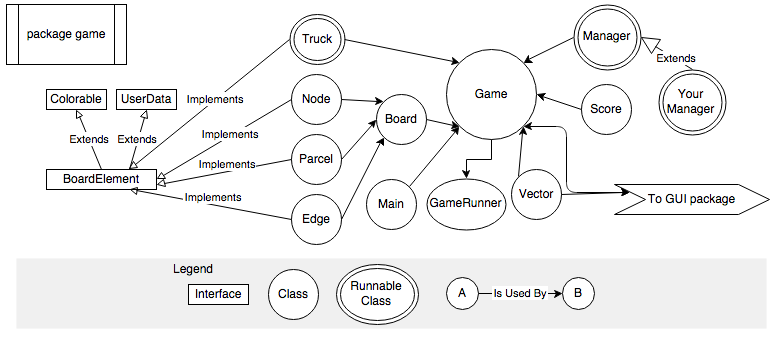
\includegraphics[scale=0.7]{hirearchy.png}} 
\caption{\em{Class Layout of package game. More lines and circles.}}
\end{figure}
\\Each interface and class in the figure is briefly explained below. For a more
thorough  explanation or the method list of a certain interface or class, see
the javadoc spec for that interface or class.
\subsection{Colorable}
The colorable interface is implemented in classes that have a "color".
Pertaining to ShippingGame, BoardElement extends Colorable so that all elements
that are drawn on the map are guaranteed to have a color.
\subsection{UserData}
The UserData interface is implemented in classes that allow the user (Your
Manager) to store data in them. You don't have to use this feature of classes
that implement UserData, but it may prove useful in some graph algorithms.
\subsection{BoardElement}
In addition to being a concatenation of the requirements of the Colorable and
UserData interfaces, the BoardElement interface specifies required behaviors for
displaying an object on the GUI. Implementing classes are required to be able to
provide various GUI-sensitive information, such as how to draw it, what it's
name on the GUI is, and if there are any trucks currently "on it".
\subsection{Truck}
Instances of the Truck class are the game pieces of ShippingGame. Trucks take
instructions from Managers, are able to travel the map and pick and drop off a
single parcel at a time. Trucks are runnable - each instance of truck is set to
run in its own thread.
\subsection{Node}
Instances of the Node class make up the Board. Each Node in the map represents a
city that is connected to other cities by highways (Edges). Nodes store parcels
until a truck picks them up. One special Node is designated as the TruckDepot,
where all Trucks begin the game and must return to before the game can end.
\subsection{Edge}
Instances of the Edge class connect the Nodes in the Board. Each Edge represents
a highway that connects two cities (Nodes). Edges in ShippingGame are undirected
(bidirectional) and weighted (have length). The weight of the edge tells how
long it takes for a truck to travel a given Edge - higher weight takes longer to
travel.
\subsection{Parcel}
Instances of the Parcel class are the scoring pieces of ShippingGame. Parcels
start at a certain Node on the Board, and award points when they are
successfully delivered to their destination Node. The game can only end once all
of the Parcels have been delivered.
\subsection{Board}
The Instance of the Board for each game stores the Nodes, Edges, and Parcels
associated with the game. It has the scoring constants related to various
actions taken during the game, and convenience methods such as getting a random
Node or random Edge.
\subsection{Score}
The Instance of Score for each game encapsulates the score for the game. In
addition to preventing the user (Your Manager) from altering the score, it has
convenience methods for checking for a valid color and calculating the cost of a
given Truck Speed.
\subsection{Vector}
The Vector class is very similar to the Point class built into java, except that
it allows for doubles in all of its calculations rather than restricting to
integers. It is used internally for calculation and is provided to you for
convenience.
\subsection{Main}
The Main class begins execution of the game, and stores static convenience
methods for use all over the project.
\subsection{Manager}
The Manager class is abstract - it is up to you to extend it. The non-abstract
behavior of the Manager class gives convenience methods for getting the map,
trucks, and parcels associated with the game. It also gives the Notification
enum, which specifies the different reasons a Truck would notify the Manager of
a change.
\subsection{Game}
An instance of the Game class represents the game as a whole. The game class is
the unifying factor that ties all of the other pieces together, along with
communicating with the GUI to make sure the visual version of the game is up to
date. It includes convenience methods for querying the current state of the
game.
\subsection{Game Runner}
An instance of the Game Runner class allows the automatic running of many games.
This is useful to automatically test your manager on may different board, and
can be accessed via arguments given to main.
\subsection{Your Manager}
An instance of Your Manager fills in the missing behavior of the Manager class
to determine how the game runs. See the next section for more on what you have
to do in your extension of the Manager class.

\newpage
\section{6. Your Tasks}
In order to complete the assignment, your primary task is write a class
extending the abstract Manager class explained in the previous section. In order
to do this, you will have to override and implement the two abstract methods
declared in the Manager class: \textbf{run()} and
\textbf{truckNotification(Truck t, Notification message)}. These two methods
determine the behavior of the trucks in the game. On their own, trucks don't do
anything; it's up to you to instruct them.\\

\begin{figure}[h]
\centerline{
\includegraphics[scale=0.4]{fry.jpg}} 
\caption{\em{The average intelligence of your shipping boys}}
\end{figure}

run() is called by the game as soon as the game begins, and allows you to do
initial computation and give your trucks their initial set of instructions.
Additionally, the body of run() will run in a separate thread from all of the
trucks, so you can continue to do computation after the trucks have begun their
travel. Your implementation can either loop forever and continually add
information to the trucks or execute a single time for initial instructions and
then rely on the truckNotification method for further interaction.\\

truckNotification(Truck t, Notification message) is called by trucks whenever
they do something of note. For a full list of the reasons why a truck would call
this method, see Manager.Notification in the previous section and in the
javadoc. This method is called by the truck in its own thread in order to ask
for more instructions. For example, upon arrival at a new node in the graph, the
truck may send a notification that there is at least one parcel at the current
node. Perhaps you want that truck to pick up that parcel before continuing on
its route.

\newpage
\section{7. Concurrency}
Because every Truck you are interacting with exists in its own thread, Shipping
Game is inherently multithread. Your manager has to be able to handle multiple
trucks calling truckNotification concurrently, without crashing or giving
incorrect instructions. That said, depending on the complexity of your solution,
you may not need to worry about concurrency at all. For example, consider the
following pseudo-code approach to the shipping game problem.
\begin{algorithm}
\caption{Basic Preprocessing} \label{alg:ls}
\begin{algorithmic}[1]
\FOR{Parcel p}
\STATE Choose arbitrary truck $t$ to deliver $p$. Store $p$ in a data structure
in $t$'s user data.
\ENDFOR
\end{algorithmic}
\end{algorithm}
\begin{algorithm}
\caption{Basic Truck Notification ($t$)} \label{alg:ls}
\begin{algorithmic}[1]
\IF{Preprocessing not done}
\STATE Return
\ENDIF
\IF{Undelivered Parcel in game}
\IF{$t$ holding parcel}
\STATE Route $t$ to its parcel's destination, then drop off the parcel
\ELSE
\STATE find the next parcel assigned to $t$, route to that parcel.
\ENDIF
\ELSE
\STATE Route $t$ home
\ENDIF
\end{algorithmic}
\end{algorithm}
\\This algorithm makes use of every truck, but because there are no data
structures that are accessed by multiple trucks and all internal data structures
are guaranteed to be thread-safe, there is no need for worry over currency.
Assuming no errors, a correctly implemented version of this algorithm  would
probably net at minimum a good grade, likely higher.\\

If, however, you're shooting for a perfect grade, you may have to do some amount
of work to ensure that your complex network of information sharing between
trucks remains thread safe. Concurrent modifications of most data structures
cause incorrect states, usually leading to null pointers or array index OOB
errors. Failure to write thread safe code might lead to unpredictable and
catastrophic errors.\\
\begin{figure}[h]
\centerline{
\includegraphics[scale=0.65]{collision.png}} 
\caption{\em{Don't rely on Spongebob to keep your code thread safe.}}
\end{figure}
\\In this vein, you have a few different options to keep code thread-safe. The
more powerful the tool, however, the greater the possibility of creating new and
more difficult problems. Ideally, come up with a strategy, than pick the
least-comprehensive tool that gives you just enough capability to prevent
potential thread safety problems.
\subsection{Approaches to Concurrency}
\begin{itemize}
\item \textbf{wait() and notify()} - Power: medium. Possibility for Error: very
	high.\\
	Java's built-in concurrency system. Threads are able to cause themselves to
	wait, using any object as a key, and to "wake up" other threads waiting on a
	given object. Working out a system of wait() and notify() calls that
	correctly limits thread movement is surprisingly difficult. At the end of
	the day, there are higher level systems that are able to accomplish the same
	tasks in a much more safe way. Don't use these unless you really want to get
	your hands dirty.
\item \textbf{Synchronized Collections} - Power: low. Possibility for error:
	none. \\
	The collection class
	\href{http://docs.oracle.com/javase/7/docs/api/java/util/Collections.html\#synchronizedCollection(java.util.Collection)}{({\color{blue}\underline{API}})}
	provides the ability to create a synchronized collection (or synchronized
	set, list, map, etc...). These collections are inherently thread-safe for
	basic operations, including adding elements, removing elements, getting
	elements, and checking the size of the collection. Notably, you can't
	iterate over a synchronized collection without a synchronized block (see
	next section), so complex operations that require iterating aren't safe. If
	you can get away with just using Synchronized Collections, you should do so
	and won't have any problems.
\item \textbf{Synchronized Blocks} - Power: medium. Possibility for Error:
	low.\\
	A synchronized block limits one thread to executing its body at a time.
	Other threads wait on before the statement until the executing thread
	finishes the block. Moreover, each synchronized block is called on some
	object in the form:
\begin{lstlisting}[frame=single]
synchronized(obj){
//...Do things that only one thread should be doing.
}
\end{lstlisting}
And only one thread can access any synchronized block that is associated with
that block at a time. This means that if there are two synchronized blocks with
the same object:
\begin{lstlisting}[frame=single]
synchronized(obj){
processA();
}
synchronized(obj){ //Note - synchronized on same obj
processB();
}
\end{lstlisting}
processA() and processB() could not possibly be executed concurrently, because a
thread's presence in one of the two blocks prevents other threads from being in
either of the two blocks.\\
The simplest way to use synchronized blocks on Synchronized collections to allow
iteration
\href{http://docs.oracle.com/javase/7/docs/api/java/util/Collections.html\#synchronizedCollection(java.util.Collection)}{({\color{blue}\underline{See
API}})}. That way only one complex (iterative) process can occur on the
collection at a time, and nothing can go wrong. \textbf{This combination is
probably the best solution for this project, and should be considered first}.
\item \textbf{Locks and Locking} - Power: High. Possibility for Error: High\\
Locks (and Semaphores and other equivalent classes) take the two pieces of a
synchronized block - preventing other threads from accessing code, and letting
other threads know that the going is clear - and separate them into two
individual lines of code. Only one thread can "own" a mutex at a time
(semaphores are generalized to allow N threads), so when a thread acquires a
Lock l, all other threads that attempt to call l.lock() are forced to wait until
the thread that owns the lock calls l.unlock(), at which point an arbitrarily
chosen thread that is waiting will call l.lock() and proceed. This gives you the
ultimate control over which threads execute what where and when, but is very
prone to issues such as deadlock in which two threads are each waiting to
acquire a lock owned by the other. These are overkill for all but the most
complex solutions, and most likely not necessary for this project. 
\end{itemize}

\newpage
\section{8. Project Schedule}
In an effort to encourage gradual progression through the project (rather than
back-ending the whole thing), the project is due in two parts. The Heap section
of the project will be due midway through the project, and the full project due
at the end. You can continue to work on and change your heap code after the heap
portion is due to improve its use in the project as whole, but the submitted
heap is the one that will be graded for heap points.

Bold lines are required, submission dates. The date of prelim 2 is included to
help in your planning. Try to at least start the heap section before you start
studying for prelim 2.\\

\begin{center}
\begin{Large}
\begin{tabular}{| c | c |}
\hline
Date & Project Milestone\\
\hline
Thursday 11/13 & Project Released\\
Thursday 11/20 & Prelim 2\\
\textbf{Sunday 11/23 @ 11:59PM} & \textbf{Heap Section Due}\\
\textbf{Thursday 12/4 @ 11:59PM} & \textbf{Full Project Due}\\
\hline
\end{tabular}
\end{Large}
\end{center}


\end{document}
